\documentclass{article}
\usepackage[utf8]{inputenc}

\usepackage{natbib}
\usepackage{graphicx}
\usepackage{fancyhdr}

\pagestyle{fancy}
\fancyhf{}
\fancyfoot[L]{Unless otherwise specififed, all content is the author's summary of "Goodfellow, Ian, Yoshua Bengio, and Aaron Courville. Deep learning. MIT press, 2016."}

\title{Adversarial Training}
\author{yusuf.roohani }
\date{August 2017}

\begin{document}
\maketitle

\section{Intriguing properties of nerual networks \cite{DBLP:journals/corr/SzegedyZSBEGF13}}

Deep neural networks are able to learn uninterpretable solutions - giving them coutner-intuitive properties. 
\begin{itemize}
    \item No distinction between high level units and linear combinations of high level units. So the space has the semantic information in the high layers of the neural network.
    
    \item DNNs learn input-output mappings that are fairly discontinuous . Can identify an adversarial example (often a hardly perceptible perturbation) by maximizing the network's prediction error. Interestingly, this doesn't seem to be a random artifact of training and can also lead to a misclassification in another network.
\end{itemize}

\section{Adversarial example detection with convolution filter statistics \cite{DBLP:journals/corr/LiL16e}}

Really interesting implementation of a model that "knows what it knows". Granting machine learning models the ability to abstain

\section{Generative Adversarial Networks}

\subsection{Learning from Simulated and Unsupervised Images using Adversarial Training \cite{shrivastava2016learning}} 

Learning from synthetic images often does not achieve the desired performenace due to a gap between synthetic and real image distributions. 

\begin{itemize}

    \item Propose simulated + unsupervised learning that uses unlabelled real data to refine synthetic images
    \item Train a refiner network to add realism to synthetic images using a combination of adversarial and self-regularization loss
    \item Modify GAN to stabilize training and reduce artifacts
    \item Show improved realism and state-of-the-art results on training deep neural networks

\end{itemize}

\section{Springenberg 2016}

\subsection{GANs}

Let $\chi = {x^1, x^2 ... x^N}$

The GAN objective could be written as:
$ \min_{G} \max_D $

\subsection{CatGANs}

Trying to learn a discriminative classifier using GAN's that calssifies inputs into multiple classes as opposed to a single class.

This is similar to a probabilitic cluster assigment but by using a discriminator trained 'adversarially', it will hopefully become more robust against overfitting to noise

The second observation is that a standard GAN cannot solve this multiclass problem - because it is only trained for a binary classification. In principle, it would learn a feature representation that could prove useful for extracting classes in future. However, important to remember that the GANs training process focusses on input features that are not correctly modeled by the generator. These features may not necessarily align with our concept of classes that we want to separate the data.

\subsection{Results}

\begin{itemize}

\item k-means:
Fails due to the euclidean distance measure it employs to evaluate distances between data points and cluster centers

\item RIM: he objective function only specifies that the deep network has to
separate the data into two equal classes, without any geometric constraints 4

\item CatGAN: the discriminator has to place its decision boundaries such that it can easily detect a non-optimal adversarial generator which seems to coincide with the correct cluster assignment. Additionally, the generator quickly learns to generate the datasets in all cases.

\end{itemize}

\subsection{Implementation}

The generator and discriminator are parametrized through neural networks

\section{SegNet}

The main motivation for SegNet was to design a road scene segmentation algorithm that would be computational time and memory efficient.


\subsection{Architecture}
Segnet consists of an encoder followed by a decoder and finally a pixelwise classification layer. The encoder architecture is VGG without FC designed for object classification. Each encoder layer has a corresponding decoder layer. Final decoder output is fed to a softmax classifier to produce class probabilities for each pixel independently.

Max pooling indidces during encoding are stored and can be resused during decoding.

The output of the softmax is a k channel image of probabilities where each channel corresponds to a specific class.

\begin{figure}
    \centering
    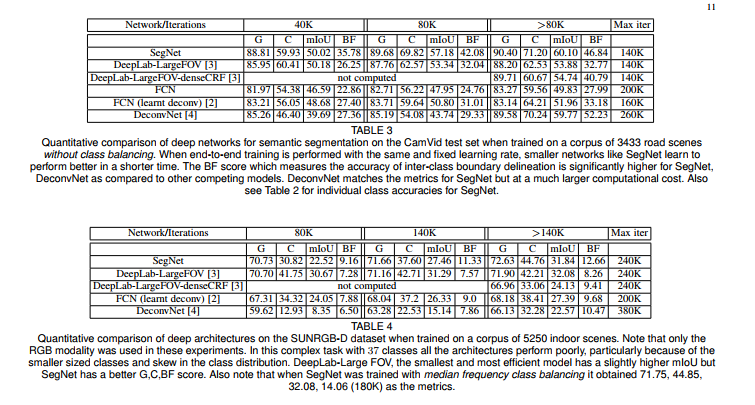
\includegraphics[scale=0.5]{Segmentation_comparison.PNG}
    \caption{Comparison of segmentation approaches using DL}
    \label{fig:my_label}
\end{figure}

\section{U-Net}

\bibliographystyle{plain}
\bibliography{references}

\end{document}